\subsection{Trigonometric Ratios}

\subsubsection{Right Angle Trigonometry}
\centerline{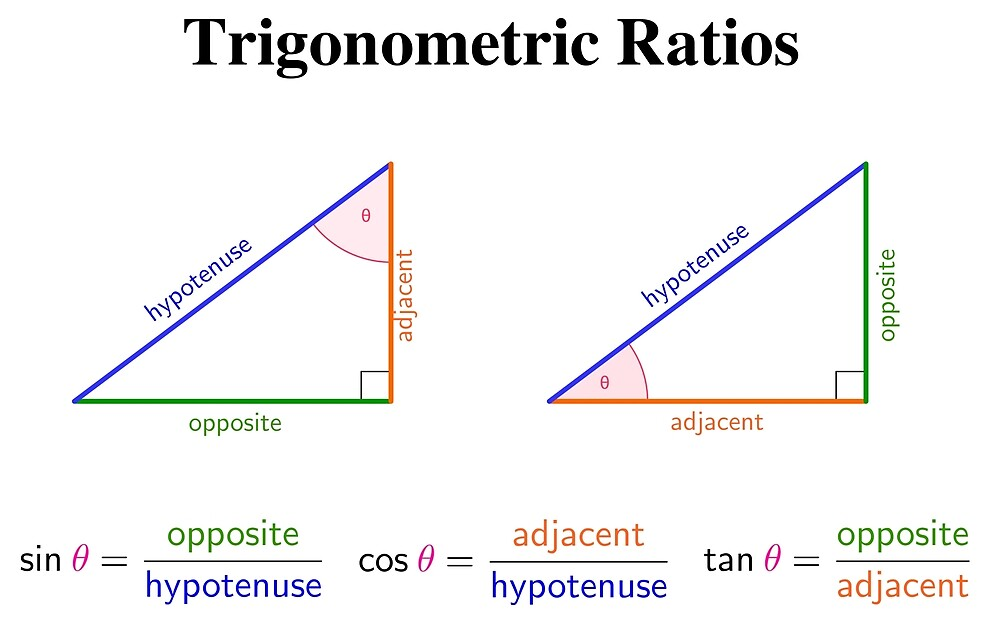
\includegraphics[scale=0.3]{Images/FundamentalsPictures/TrigRatios.jpg}}
Hypotenuse is the lonest end of the triangle.\\
Opposite is the side across from the angle in question.\\
Adjacent is the side next to the angle in question.\\
Note these ratios only work for right angle triangles.\\
\\
Special Triangles:\\
Often we need a calculator to determine the numeric value of the side lengths. There are two useful triangles that we use that allows us to compute the trig ratios without using a calculator. These are called special triangles.\\
\centerline{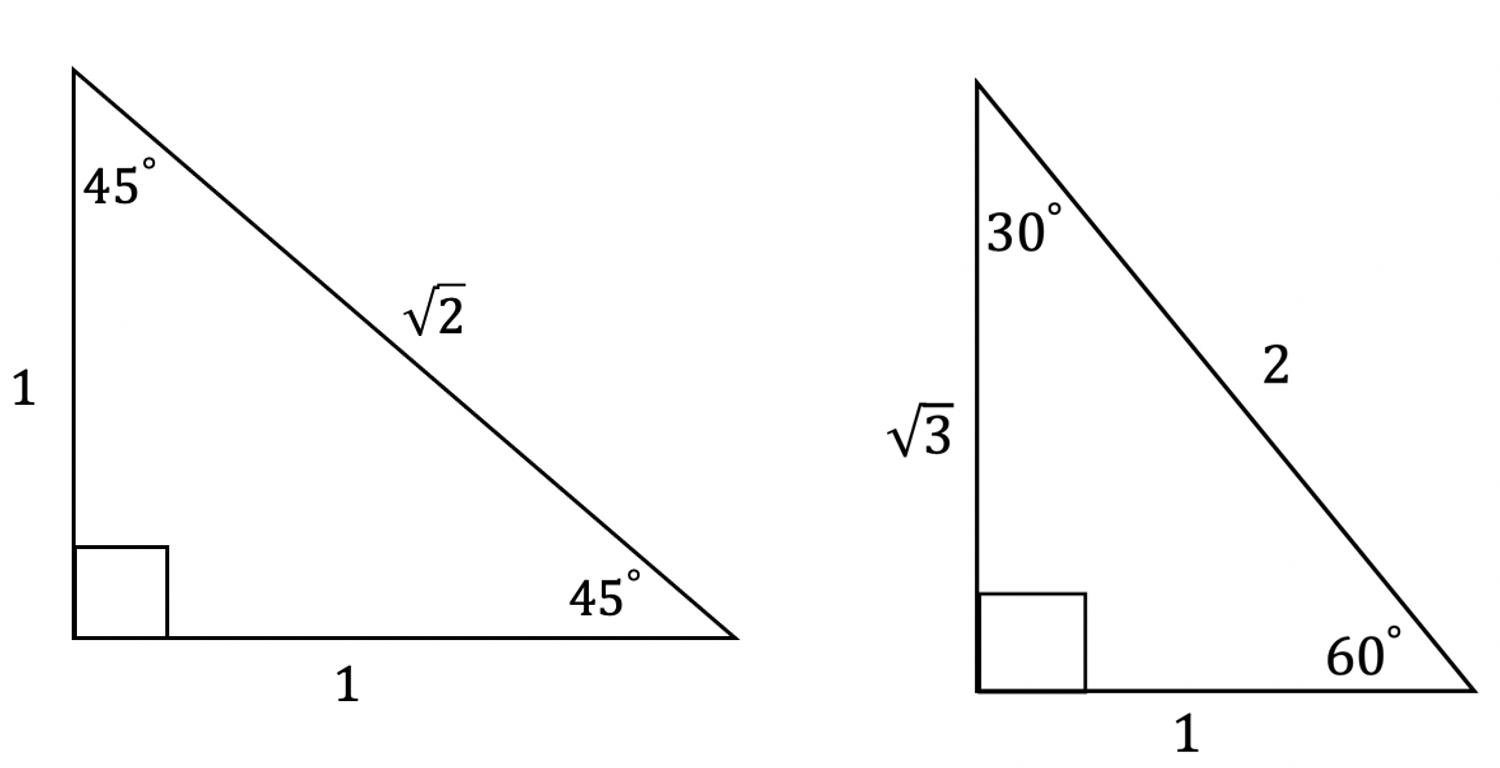
\includegraphics[scale=0.5]{Images/FundamentalsPictures/SpecialTriangles.png}}

\subsubsection{Sine and Cosine Law}
\centerline{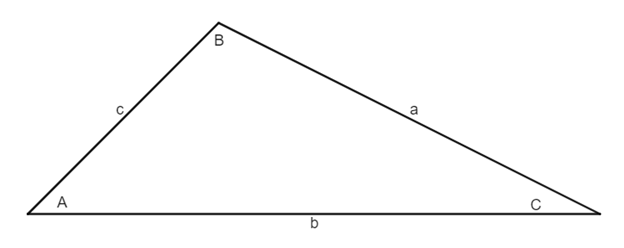
\includegraphics[scale=0.7]{Images/FundamentalsPictures/SineLawTriangle.png}}
The cosine law is an extension of Pythagorean's theorem for all triangles (not just right angled ones).
$$c^2=a^2+b^2-2ab\cos C$$
Note that the usage of $a$, $b$, and $c$ is interchangeable.\\
\\
The sine law is a relationship between the ratio of sides and angles in any triangle.
$$\frac{\sin A}{a}=\frac{\sin B}{b}=\frac{\sin C}{c}$$